\documentclass[border=6pt]{standalone}
\usepackage{tikz}
\usetikzlibrary{positioning,arrows.meta,calc,decorations.pathreplacing}
\usepackage[scaled=0.95]{helvet}
\renewcommand{\familydefault}{\sfdefault}
\definecolor{ink}{HTML}{1F2328}\definecolor{muted}{HTML}{57606A}
\definecolor{cS}{HTML}{8250DF}  % Stage 1 lead-lag selector
\definecolor{cEL}{HTML}{2A78D6} % Express Links
\definecolor{cFO}{HTML}{EB6834} % Forecast-only
\definecolor{cRA}{HTML}{1BAF7A} % random
\definecolor{fast}{HTML}{2DA44E}\definecolor{mid}{HTML}{D4A72C}\definecolor{slow}{HTML}{CF222E}
\hyphenpenalty=10000
% node positions: two clusters joined by one bridge (hL -- hR)
\def\nodelist{L1/0/0.5,L2/0/-0.5,L3/0.8/1.0,L4/0.8/0,L5/0.8/-1.0,L6/1.6/0.5,L7/1.6/-0.5,hL/2.35/0,hR/3.35/0,R1/4.1/0.5,R2/4.1/-0.5,R3/4.9/1.0,R4/4.9/0,R5/4.9/-1.0,R6/5.7/0.5,R7/5.7/-0.5}
\def\edgelist{L1/L3,L1/L4,L2/L4,L2/L5,L3/L6,L4/L6,L4/L7,L5/L7,L6/hL,L7/hL,hR/R1,hR/R2,R1/R3,R1/R4,R2/R4,R2/R5,R3/R6,R4/R6,R4/R7,R5/R7}
\def\rnsize{2.6mm}
% \road{prefix}{(shift)}{scale}{fill colour}
\newcommand{\road}[4]{%
  \begin{scope}[shift={#2}, scale=#3]
    \foreach \n/\x/\y in \nodelist {\coordinate (#1\n) at (\x,\y);}
    \foreach \a/\b in \edgelist {\draw[ink!45, line width=0.6pt] (#1\a)--(#1\b);}
    \draw[ink!70, line width=1.8pt] (#1hL)--(#1hR);
    \foreach \n/\x/\y in \nodelist {\node[circle, inner sep=0pt, minimum size=\rnsize, draw=ink!75, line width=0.45pt, fill=#4] at (#1\n) {};}
  \end{scope}}
\tikzset{newlink/.style={-{Stealth[length=2.2mm]}, line width=1.4pt, #1},
         arr/.style={-{Stealth[length=2.6mm]}, line width=1pt, draw=ink!65}}

\begin{document}
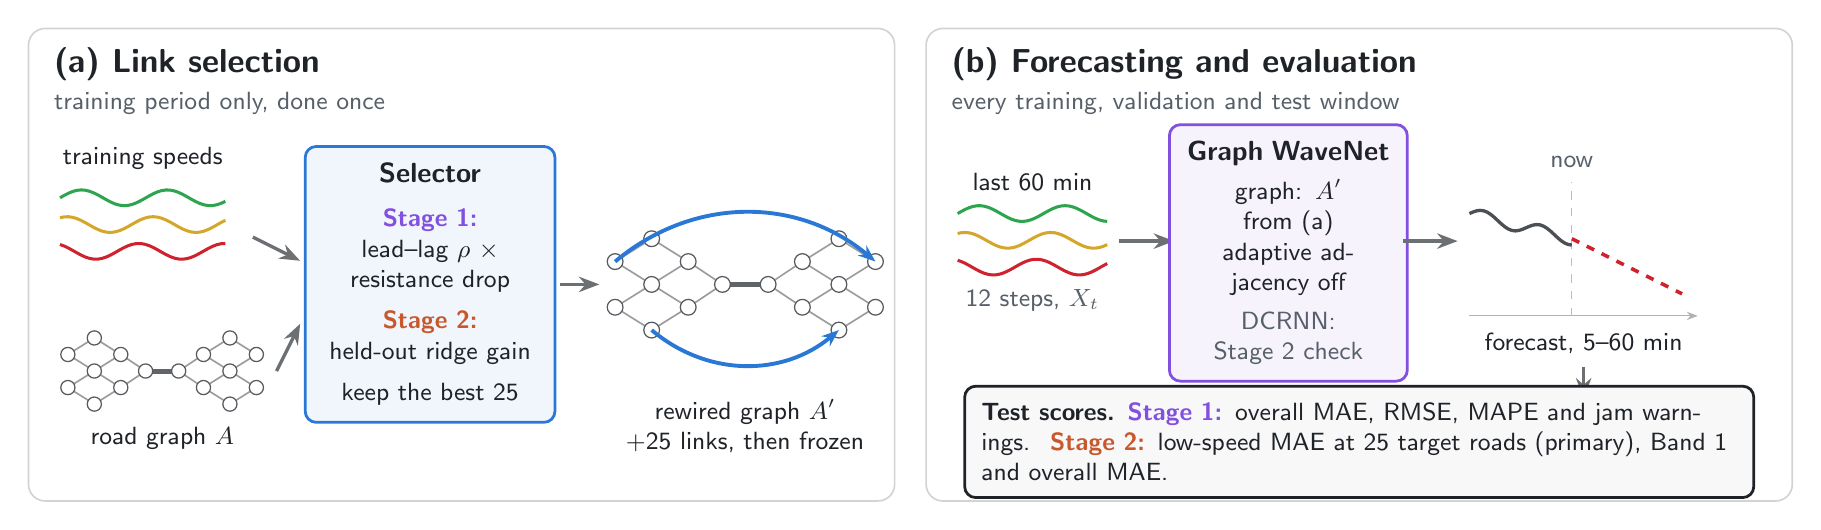
\begin{tikzpicture}[font=\normalsize, color=ink,
  blk/.style={draw=#1, fill=#1!7, rounded corners=4pt, line width=1pt, align=center, inner sep=6pt},
  panel/.style={draw=ink!20, rounded corners=6pt, line width=0.6pt},
  ptitle/.style={font=\large\bfseries, anchor=west}]

%======================== (a) link selection ========================
\draw[panel] (-0.4,-3.0) rectangle (10.6,3.0);
\node[ptitle] at (-0.2,2.55) {(a) Link selection};
\node[font=\small, text=muted, anchor=west] at (-0.2,2.05) {training period only, done once};

% inputs
\node[font=\small] at (1.05,1.35) {training speeds};
\foreach \k/\c in {0/fast,1/mid,2/slow}{
  \draw[\c, line width=1.1pt, domain=0:2.1, samples=40] plot (\x, {0.85-0.34*\k+0.1*sin(330*\x+60*\k)});}
{\def\rnsize{1.8mm}\road{ia}{(0.1,-1.35)}{0.42}{white}}
\node[font=\small] at (1.3,-2.2) {road graph $A$};

\draw[arr, line width=1.2pt] (2.45,0.35) -- (3.05,0.05);
\draw[arr, line width=1.2pt] (2.75,-1.35) -- (3.05,-0.75);

% selector
\node[blk=cEL, text width=2.75cm, font=\small] (sel) at (4.7,-0.25) {%
  {\normalsize\bfseries Selector}\\[5pt]
  {\color{cS}\textbf{Stage 1:}}\\ lead--lag $\rho$ $\times$ resistance drop\\[4pt]
  {\color{cFO!85!black}\textbf{Stage 2:}}\\ held-out ridge gain\\[4pt]
  keep the best 25};

\draw[arr, line width=1.2pt] (6.35,-0.25) -- (6.85,-0.25);

% rewired graph
{\def\rnsize{2.0mm}\road{rw}{(7.05,-0.25)}{0.58}{white}}
\draw[newlink=cEL, line width=1.4pt] (rwL1) to[bend left=40] (rwR6);
\draw[newlink=cEL, line width=1.4pt] (rwL5) to[bend right=40] (rwR5);
\node[font=\small\bfseries] at (9.95-0.05,1.45) {};
\node[font=\small, align=center] at (8.7,-2.05) {rewired graph $A'$\\+25 links, then frozen};

%======================== (b) forecasting and evaluation ========================
\draw[panel] (11.0,-3.0) rectangle (22.0,3.0);
\node[ptitle] at (11.2,2.55) {(b) Forecasting and evaluation};
\node[font=\small, text=muted, anchor=west] at (11.2,2.05) {every training, validation and test window};

% input window
\node[font=\small] at (12.35,1.05) {last 60 min};
\foreach \k/\c in {0/fast,1/mid,2/slow}{
  \draw[\c, line width=1.1pt, domain=0:1.9, samples=40] plot (11.4+\x, {0.65-0.34*\k+0.1*sin(330*\x+60*\k)});}
\node[font=\small, text=muted] at (12.35,-0.45) {12 steps, $X_t$};

\draw[arr, line width=1.2pt] (13.45,0.3) -- (14.15,0.3);

% forecaster
\node[blk=cS, text width=2.6cm, font=\small] (gwn) at (15.6,0.15) {%
  {\normalsize\bfseries Graph WaveNet}\\[3pt] graph: $A'$ from (a)\\ adaptive adjacency off\\[3pt] {\color{muted}DCRNN: Stage 2 check}};

\draw[arr, line width=1.2pt] (17.05,0.3) -- (17.75,0.3);

% forecast
\begin{scope}[shift={(17.9,-0.15)}]
 \draw[ink!35, -{Stealth[length=1.4mm]}] (0,-0.5) -- (2.9,-0.5);
 \draw[ink!30, dashed] (1.3,-0.5) -- (1.3,1.2);
 \node[font=\small, text=muted] at (1.3,1.45) {now};
 \draw[ink!80, line width=1.2pt, domain=0:1.3, samples=30] plot (\x, {0.8-0.25*\x+0.08*sin(500*\x)});
 \draw[slow, line width=1.3pt, dashed, domain=1.3:2.7, samples=30] plot (\x, {0.48-0.5*(\x-1.3)});
\end{scope}
\node[font=\small] at (19.35,-1.0) {forecast, 5--60 min};

% evaluation (below)
\draw[arr, line width=1.2pt] (19.35,-1.3) -- (19.35,-1.7);
\node[blk=ink, text width=9.6cm, font=\small, align=left, fill=ink!3] (ev) at (16.5,-2.25) {%
  \textbf{Test scores.} {\color{cS}\textbf{Stage 1:}} overall MAE, RMSE, MAPE and jam warnings.\;
  {\color{cFO!85!black}\textbf{Stage 2:}} low-speed MAE at 25 target roads (primary), Band~1 and overall MAE.};


\end{tikzpicture}
\end{document}
